\chapter[]{Tessuti artificiali}
\graphicspath{ {./images/chapter5/} }

\begin{figure}[h]
	\centering
		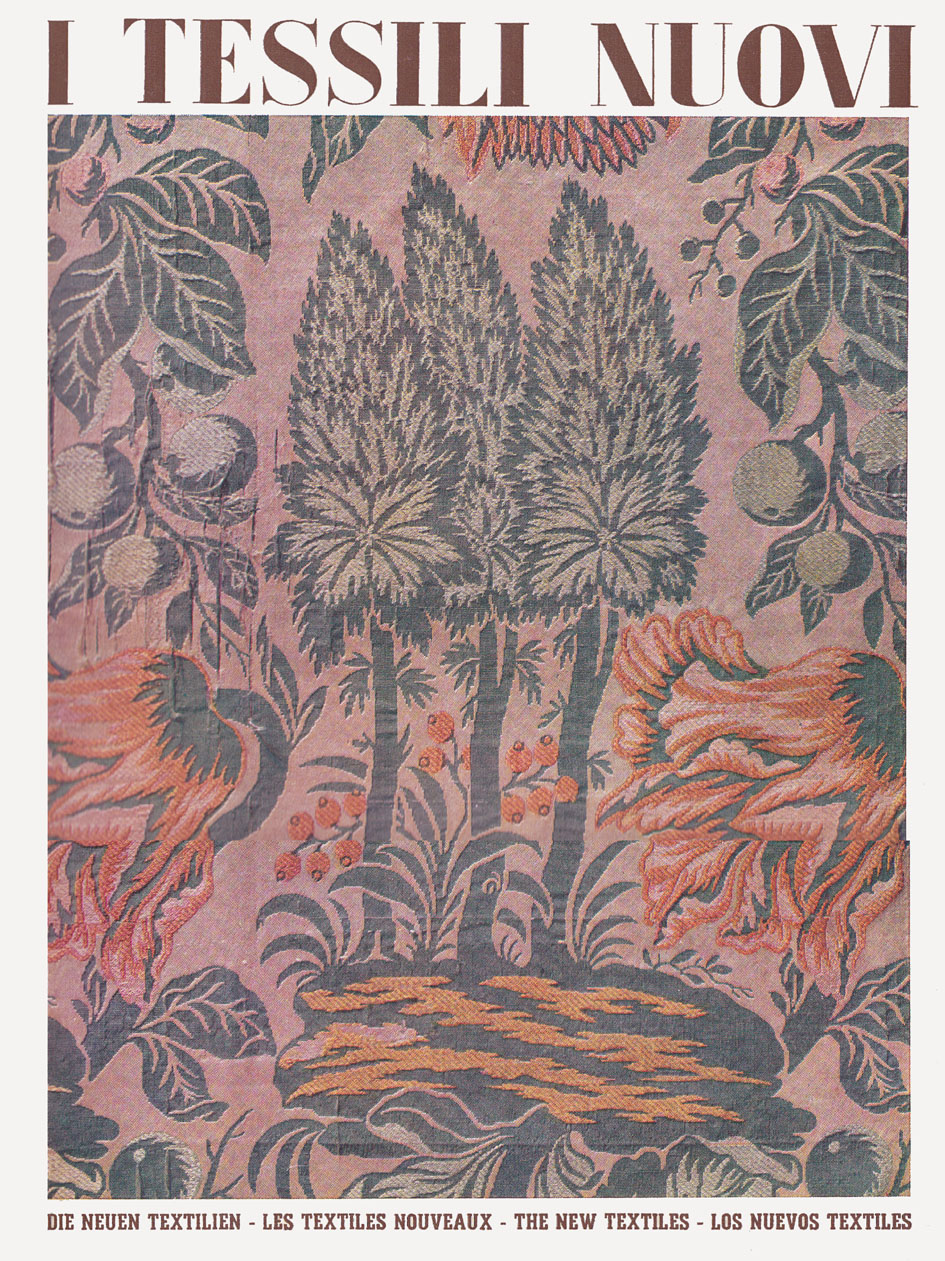
\includegraphics[width=\textwidth]{tessilinuovi.jpg}
	\caption{Copertina della rivista trimestrale “I TESSILI NUOVI” n° 28  Luglio-Settembre 1941}
	\label{fig:tessilinuovi}
\end{figure}

\newpage

   La DAF negli anni ’30 del XX° secolo era all’apice del livello produttivo sia come qualità che quantità. Ma nel 1935 con la guerra d’Etiopia l’Italia si trovò a dover contrastare l’embargo delle materie prime voluto dalla Società delle Nazioni per iniziativa di Gran Bretagna e Francia.
   Nel campo tessile per far fronte alla penuria di materiale naturale vennero incrementate al massimo la ricerca e la produzione di fibre sintetiche . 
   Venivano così prodotti dei surrogati denominati Lanital, Terital, Rayon ecc… ecc….
   Tra le aziende produttrici di tessuti con questi materiali imposti dalla autarchia vi era la Snia Viscosa. 
   Questa industria pubblicava una rivista trimestrale che informava sulle iniziative aziendali e le attività produttive. Il titolo della pubblicazione era “I TESSILI NUOVI”. 
   Dal numero 28 del Luglio - Settembre 1941 e dal numero 31 dell’Aprile – Giugno 1942 di detto periodico apprendiamo che anche la DAF utilizzava tessuti SNIA per i propri stampati.
   Sempre su questi numeri viene riferito che la grande e milanesissima Sarta (a quei tempi si nominava così chi produceva alta moda) Biki utilizzava prodotti SNIA per le proprie creazioni. Accostando questi riferimenti è lecito supporre, anche se tuttora una conferma non l’abbiamo, che Biki per i suoi  lavori usasse prodotti DAF  con materiali sia sintetici che naturali. 

\newpage

\begin{figure}[h]
	\centering
		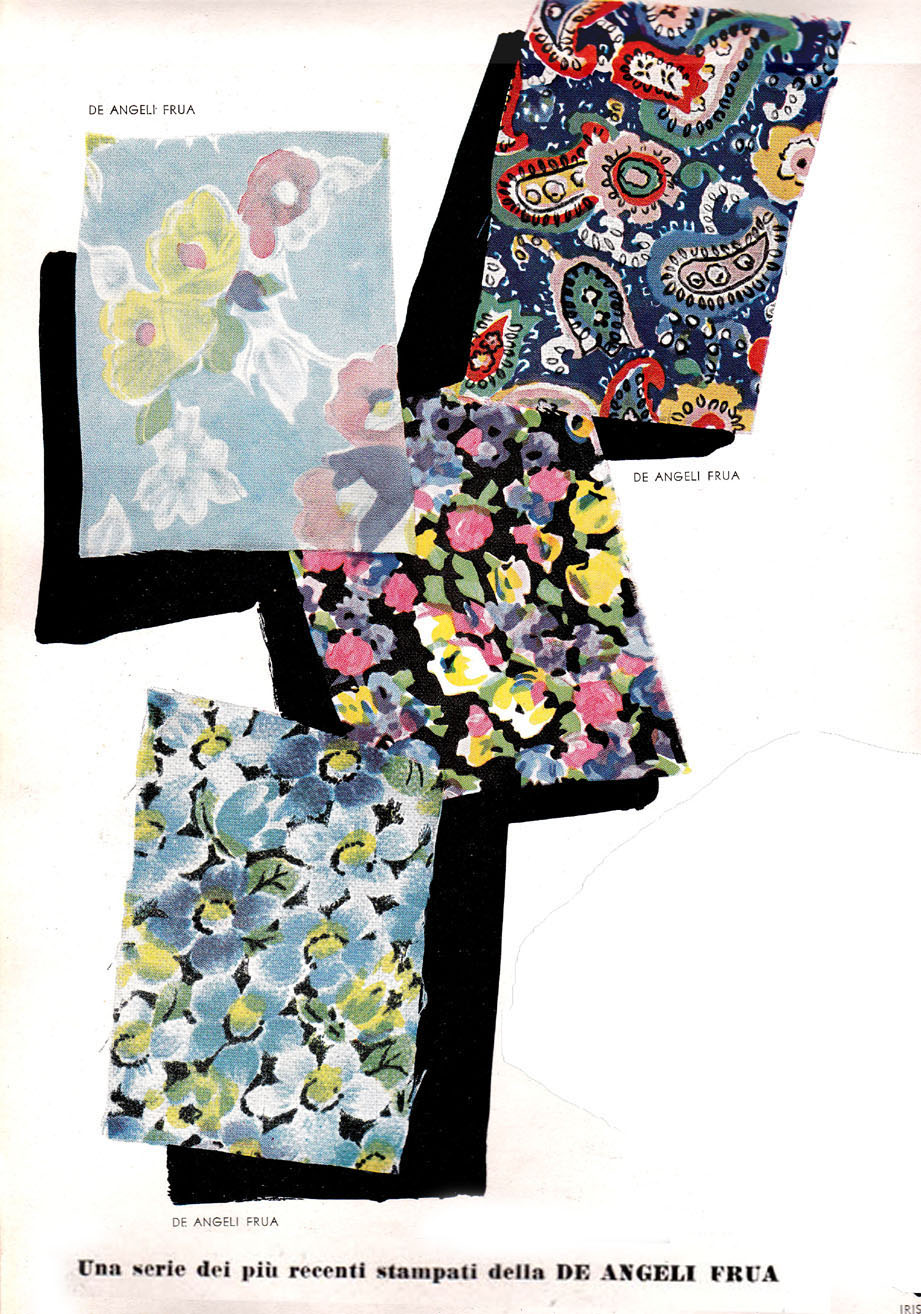
\includegraphics[width=\textwidth]{tessilinuovi_2.jpg}
	\caption{Dalla rivista “I TESSILI NUOVI” n° 28 – 1941  pag. 8}
	\label{fig:tessilinuovi_2}
\end{figure}

\newpage

\begin{figure}[h]
	\centering
		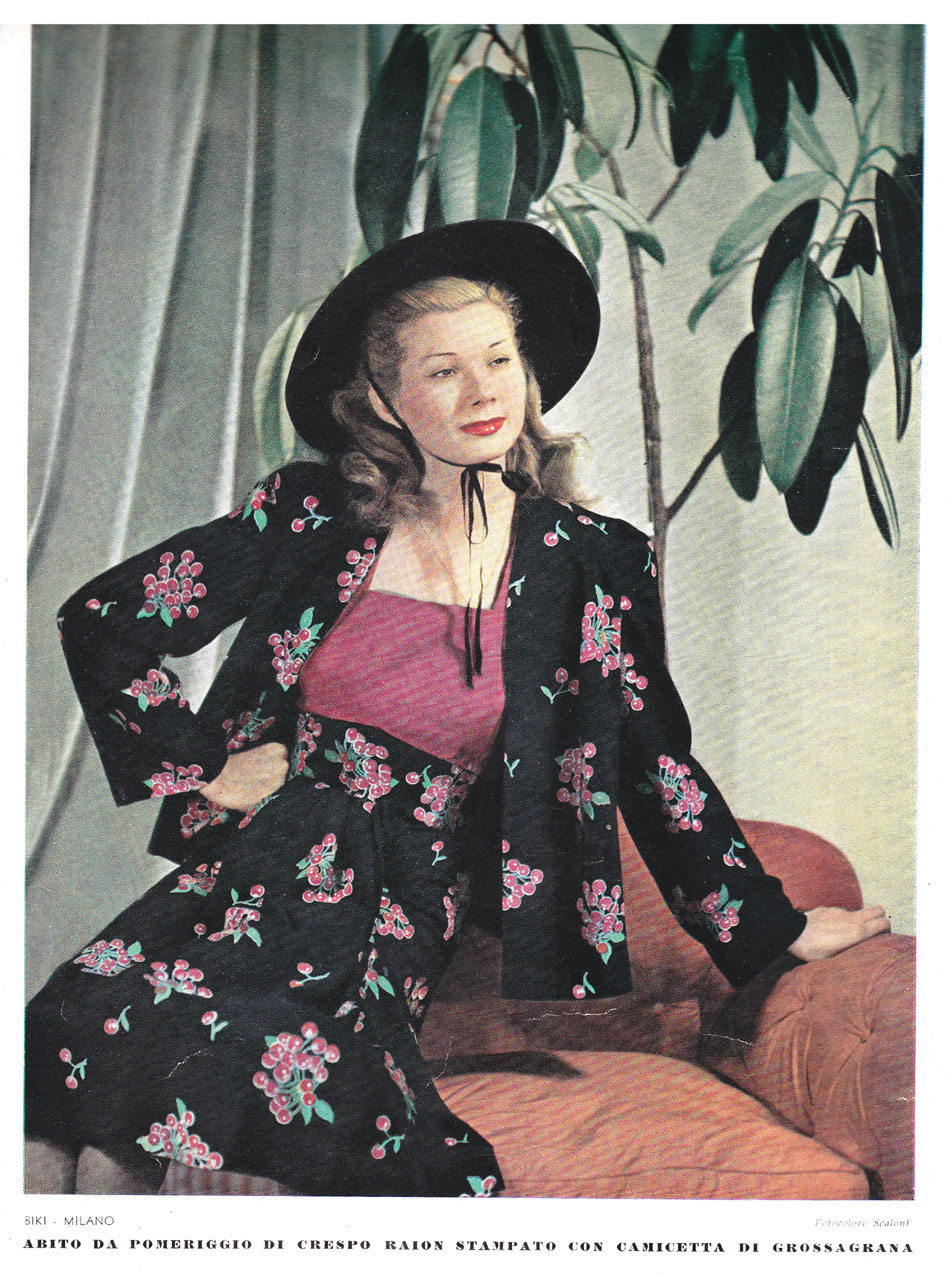
\includegraphics[width=\textwidth]{tessilinuovi_3.jpg}
	\caption{Dalla rivista “I TESSILI NUOVI”n° 31 Aprile-Giugno 1942 pag. 4}
	\label{fig:tessilinuovi_3}
\end{figure}

A piè di foto la scritta BIKI MILANO

\newpage

\begin{figure}[h]
	\centering
		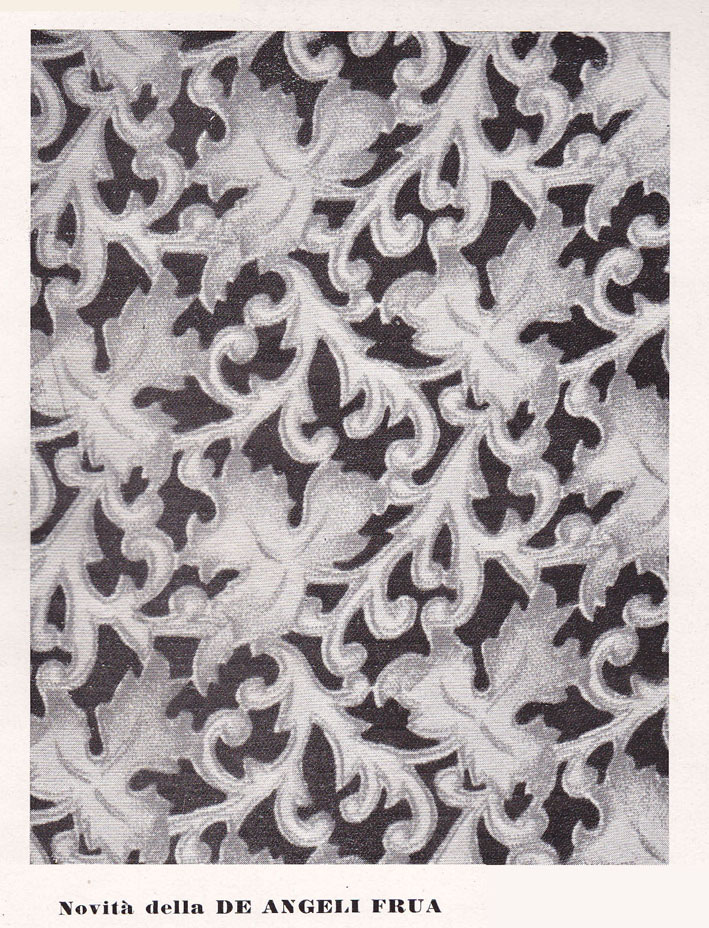
\includegraphics[width=\textwidth]{tessilinuovi_4.jpg}
	\caption{Dalla Rivista “I TESSILI NUOVI”n° 28- 1941 pag. 11}
	\label{fig:tessilinuovi_4}
\end{figure}

\begin{figure}[h]
	\centering
		
\includegraphics[width=\textwidth]{logo_snia.jpg}
	\caption{Logo  SNIA VISCOSA}
	\label{fig:logo_snia}
\end{figure}

\newpage

\begin{figure}[h]
	\centering
		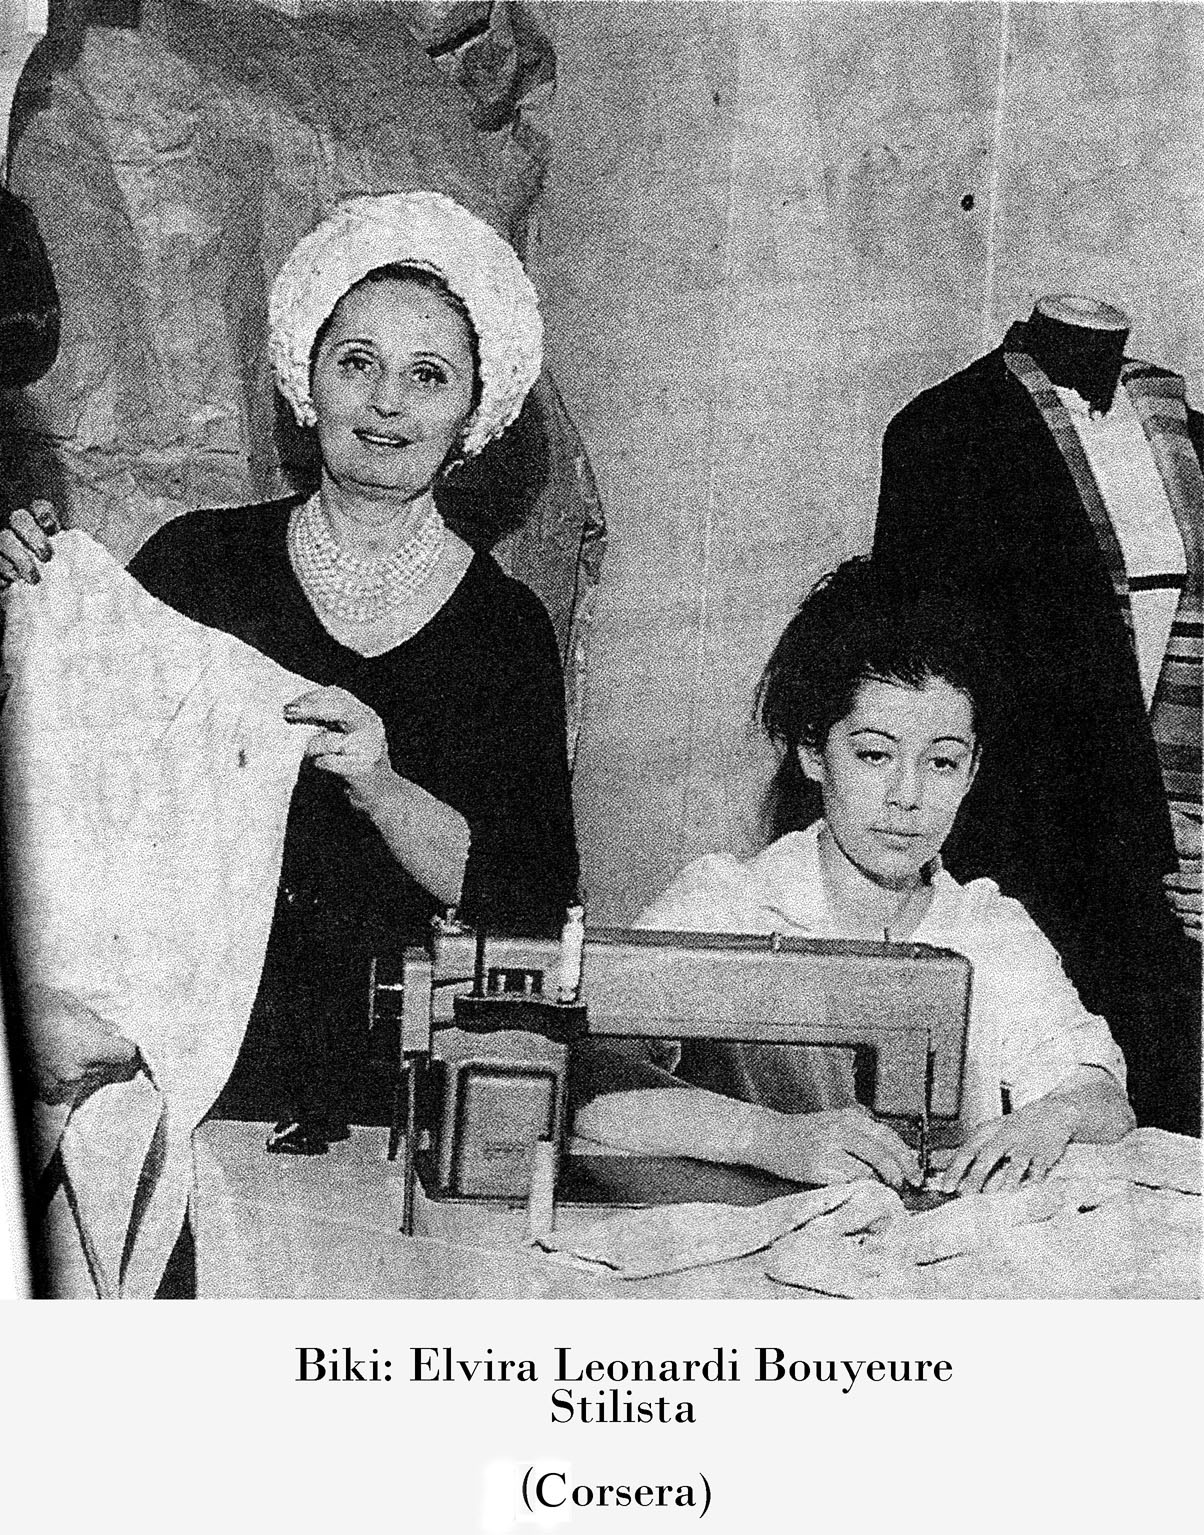
\includegraphics[width=\textwidth]{biki.jpg}
	\caption{}
	\label{fig:biki}
\end{figure}

\newpage

\begin{figure}[h]
	\centering
		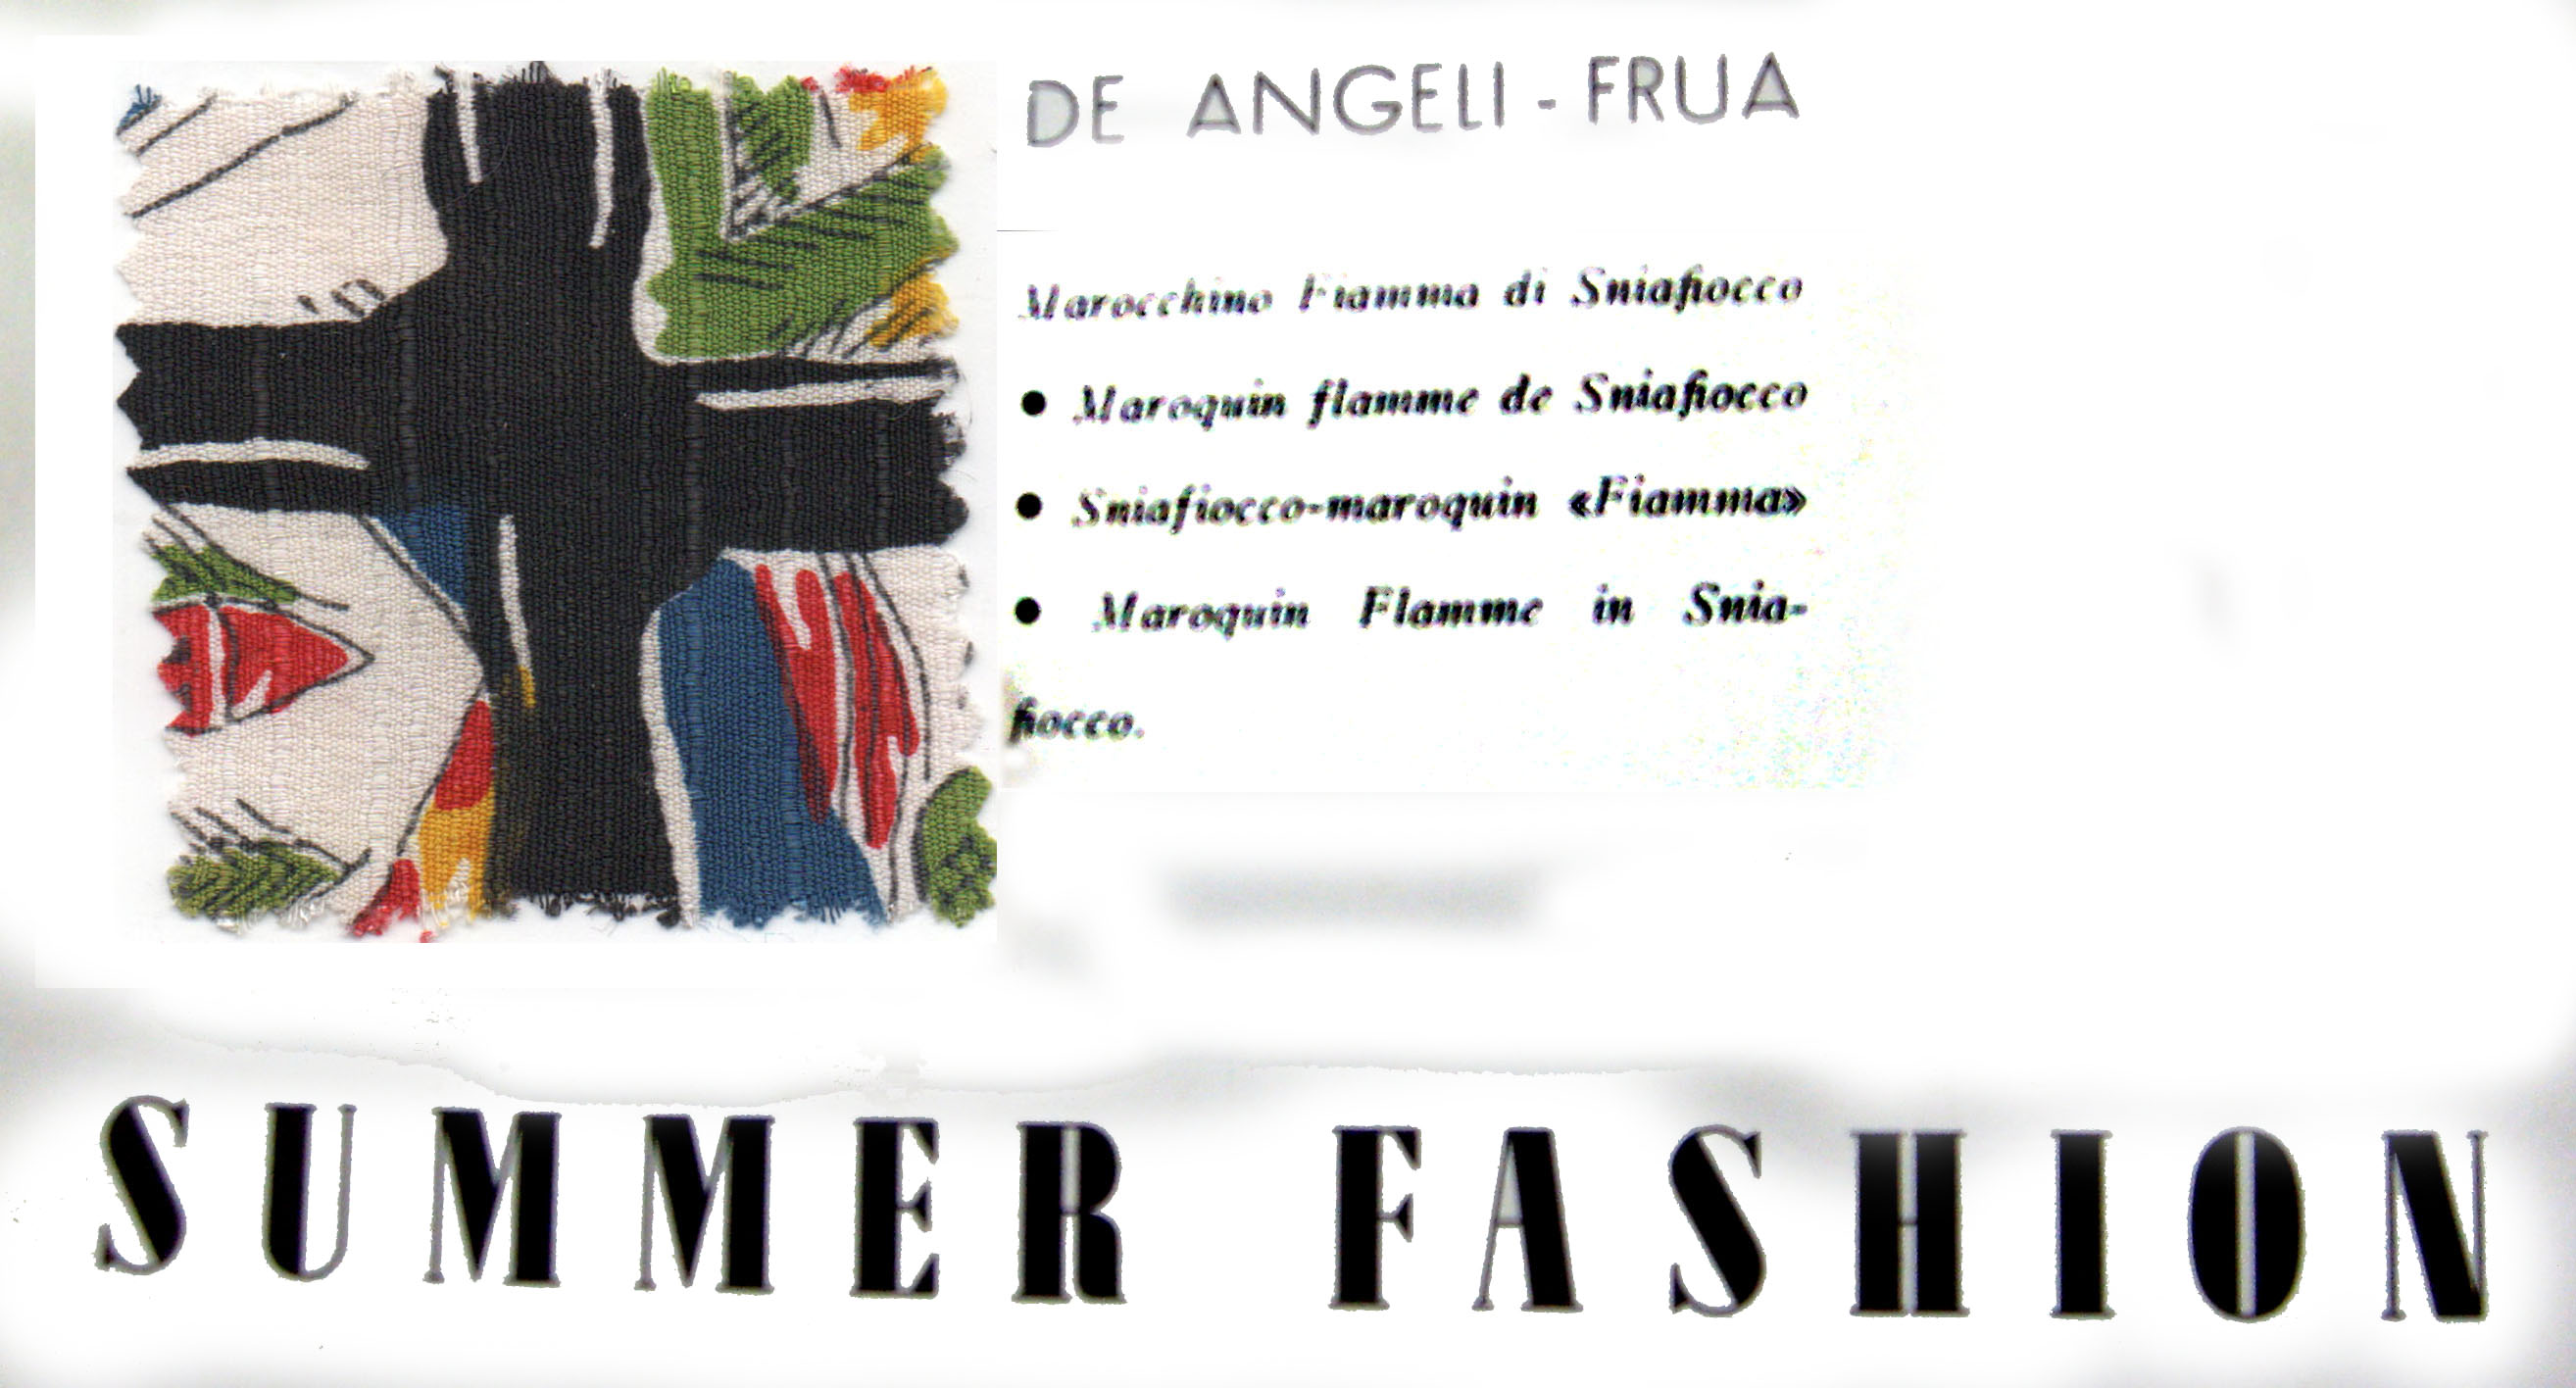
\includegraphics[width=\textwidth]{summer_fashon_1.jpg}
	\caption{}
	\label{fig:summer_fashon_1}
\end{figure}

\begin{figure}[h]
	\centering
		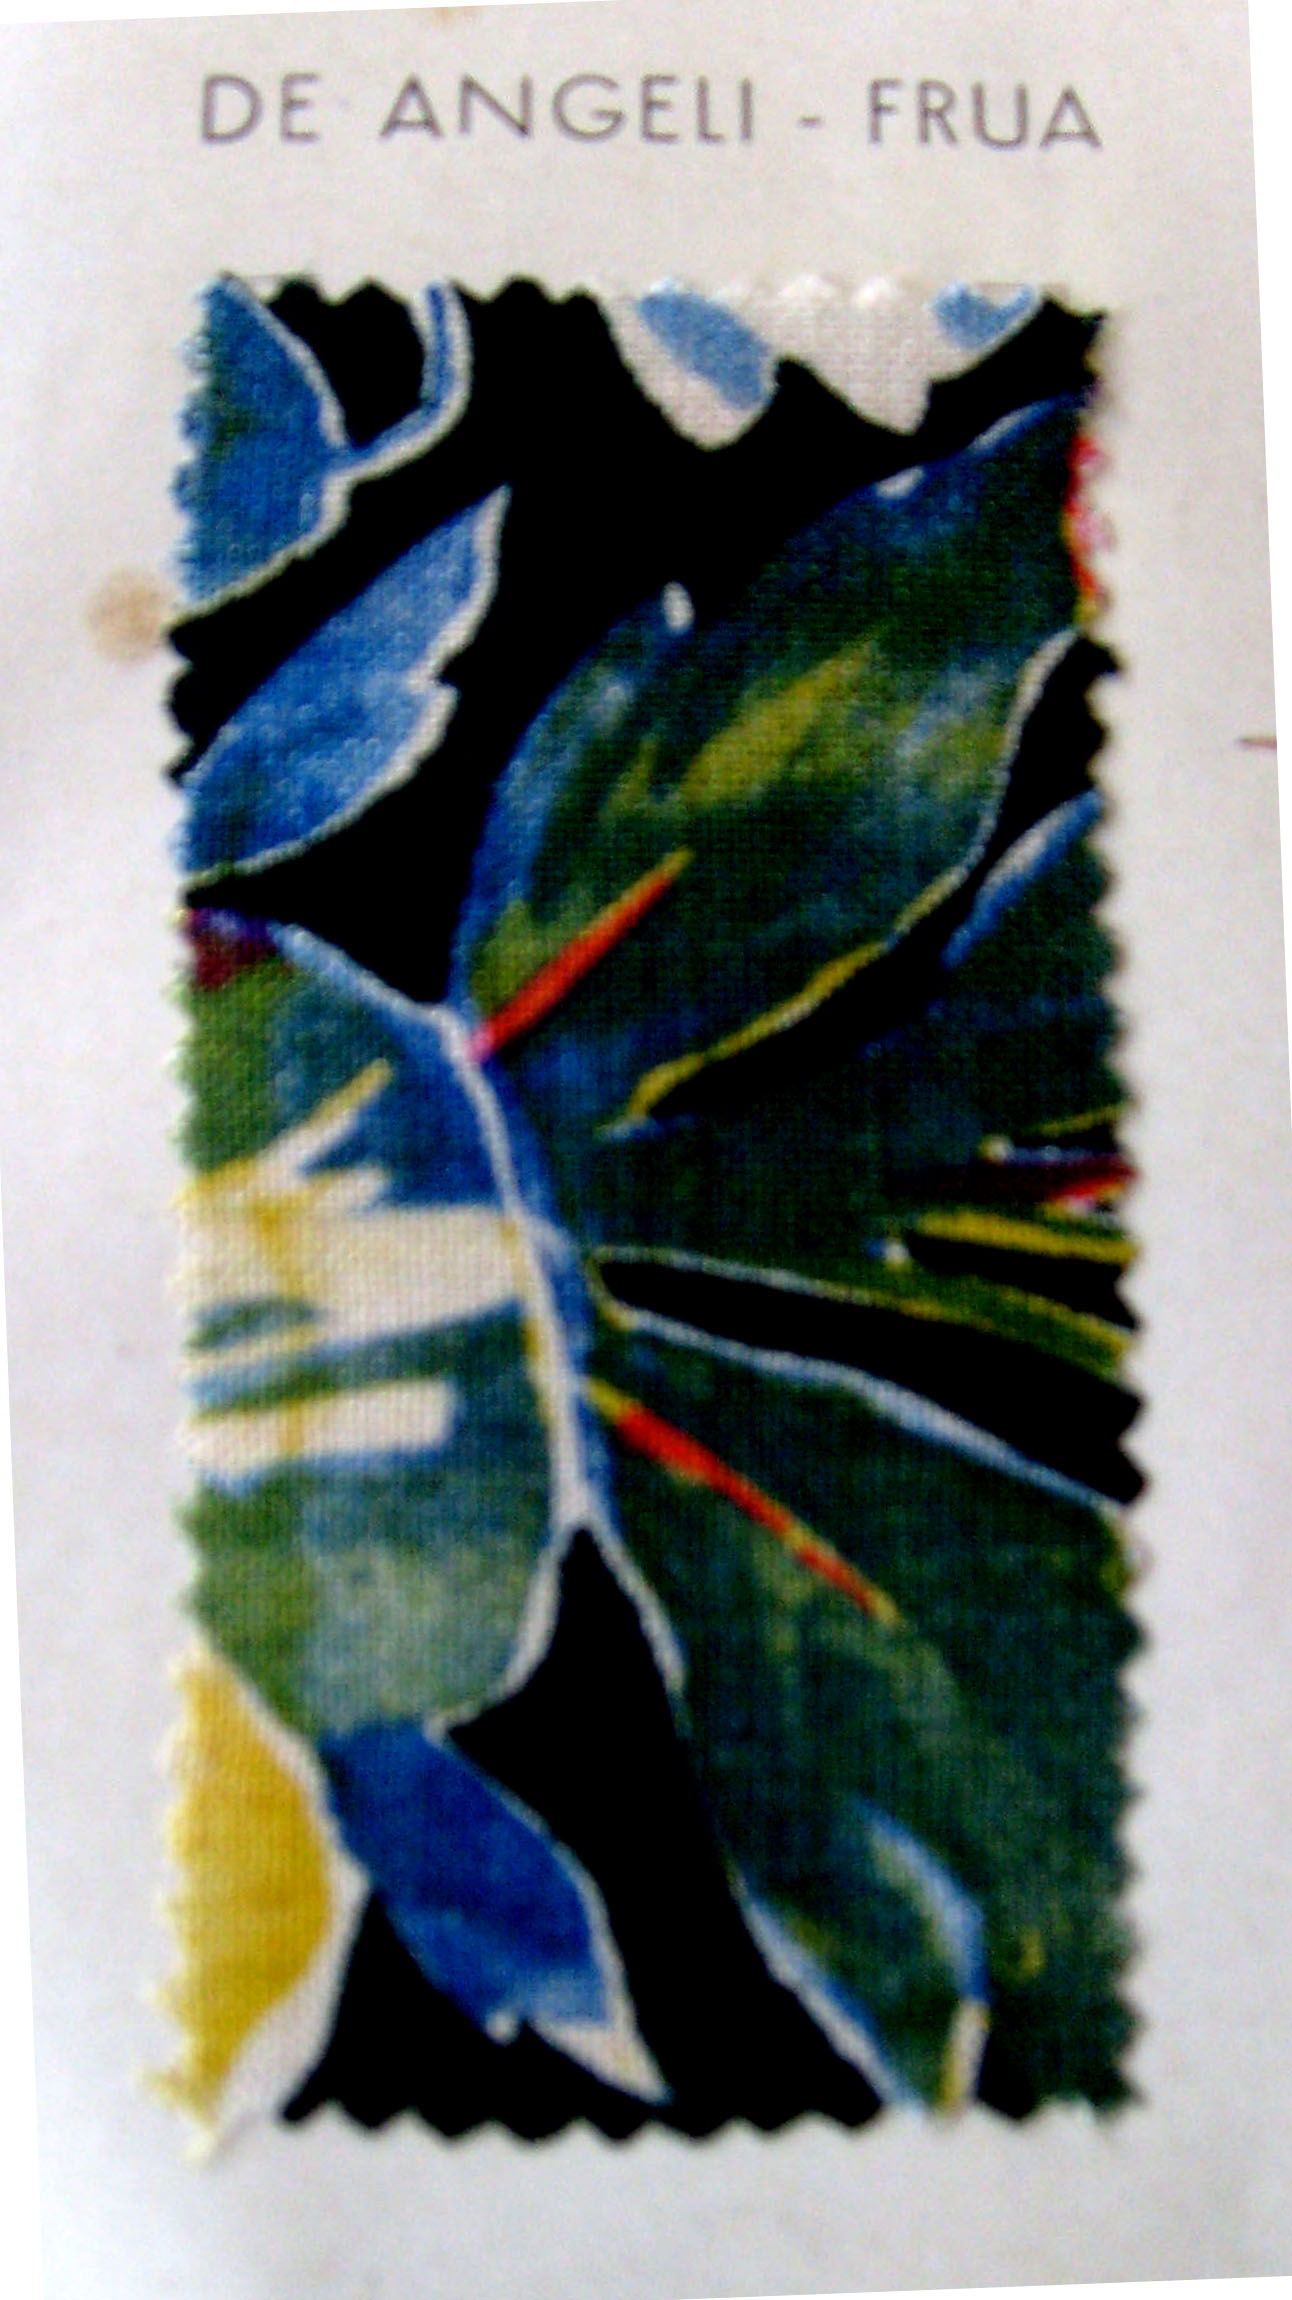
\includegraphics[width=\textwidth]{summer_fashon_2.jpg}
	\caption{}
	\label{fig:summer_fashon_2}
\end{figure}

\newpage

\begin{figure}[h]
	\centering
		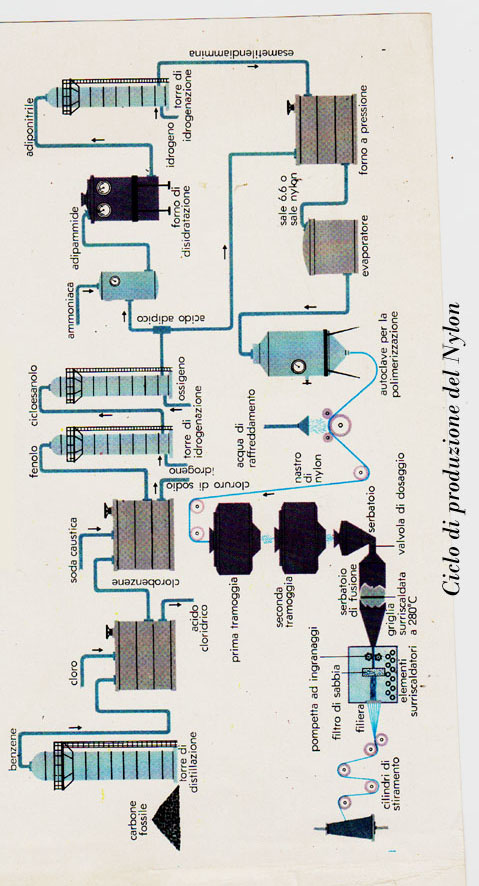
\includegraphics[width=\textwidth]{ciclo_produzione_nylon.jpg}
	\caption{}
	\label{fig:ciclo_produzione_nylon}
\end{figure}

\newpage

\begin{figure}[h]
	\centering
		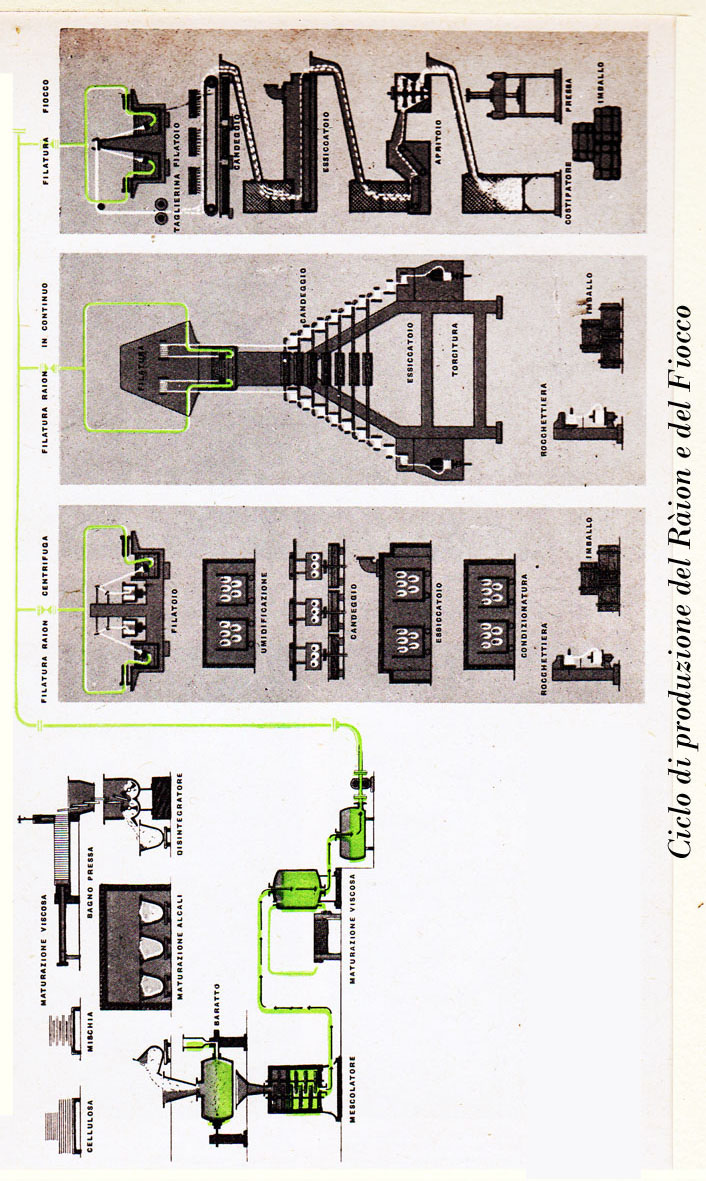
\includegraphics[width=\textwidth]{ciclo_produzione_raion.jpg}
	\caption{}
	\label{fig:ciclo_produzione_raion}
\end{figure}

\clearpage




